\section{二元关系}
\subsection{序偶}

\begin{frame}{序偶}
\pause
\vspace{-2ex}
\finger 在日常生活中,有许多事物是成对出现的,具有一定的顺序。
\pause
\begin{center}
$\cquptred{1}<\cquptred{2}$\qquad \pause
\cquptred{重庆邮电大学}位与\cquptred{南山}\qquad \pause
\cquptred{草}在结它的\cquptred{种子}
\end{center}\pause

%\begin{defi}
%  两个元素$x, y$构成的有序二元组$\opxy$,称为\alert{序偶 (ordered pair)}。通常把$\opxy$定义为
%  \[\opxy\triangleq\{\{x\},\{x,y\}\}\]
%  称$x$为$\opxy$的\alert{第一元素},称$y$为$\opxy$的\alert{第二元素}。
%\end{defi}

\begin{defi}
  两个元素$x, y$构成的有序二元组$\opxy$,称为\alert{序偶 (ordered pair)}。通常把
  $x$称 为$\opxy$的\alert{第一元素},$y$称 为$\opxy$的\alert{第二元素}。
\end{defi}

\end{frame}
%==============================================================================%
\begin{frame}{序偶}
\pause
\begin{itemize}
  \item 在集合中$\{x,y\}=\{y,x\}$, 他们是无序偶;一般的,对于序偶$\opxy\neq\langle y,x\rangle $。
\end{itemize}\pause
\vspace{2ex}
\begin{thm}
  对任意序偶$\langle a,b\rangle,\langle c,d\rangle$
  \vspace{-1ex}\[\langle a,b\rangle=\langle c,d\rangle,\quad\mbox{当且仅当~} a=c,b=d.\]
\end{thm}


\end{frame}

%==============================================================================%

\begin{frame}{有序三元组}
\pause
\begin{defi}
  \alert{有序三元组(ordered triple)}是一个序偶,其第一元素本身也是一个序偶,可形式化表示为$$\langle \opxy,z\rangle.$$约定有序三元组可记为:$\langle x,y,z\rangle$。
\end{defi}\pause
\vspace{2ex}
\begin{itemize}
  \item $\langle \opxy,z\rangle\neq\langle x,\langle y,z\rangle\rangle$,因为后者不是有序三元组。
\end{itemize}

\end{frame}

%==============================================================================%

\begin{frame}{有序$n$元组}
\pause
\begin{defi}
  \alert{有序$n$元组(ordered $n-$tuple)}$\left\langle x_1,x_2,\ldots,x_n\right\rangle$递归地定义为:
  \begin{equation*}
    \begin{aligned}
      %\left\langle x_1,x_2 \right\rangle&=\left\{\left\{x_1\right\},\left\{x_1,x_2\right\}\right\},\\
      \left\langle x_1,x_2,x_3 \right\rangle&=\left\langle\left\langle x_1,x_2 \right\rangle,x_3 \right\rangle,\\
      &\cdots\cdots \\
     \left\langle x_1,\ldots,x_{n-1},x_n \right\rangle&=\left\langle\left\langle x_1,\ldots,x_{n-1} \right\rangle,x_{n} \right\rangle,
    \end{aligned}
  \end{equation*}
  其中第$i$个元素$x_i$称为有序$n$元组的\alert{第$i$个坐标($i$th coordinate)}。
\end{defi}

\end{frame}

%==============================================================================%

\begin{frame}{有序$n$元组}
\pause
\begin{itemize}
  \item 有序$n$元组$\left\langle x_1,x_2,\ldots,x_n\right\rangle$是一个序偶,其中第一元素为有序$n-1$元组$\left\langle x_1,x_2,\ldots,x_{n-1}\right\rangle$。
\end{itemize}
\vspace{2ex}
\pause
\begin{thm}
  两个有序$n$元组$\left\langle x_1,x_2,\ldots,x_n\right\rangle=\left\langle y_1,y_2,\ldots,y_n\right\rangle$ 当且仅当
  \[x_1=y_1\land x_2=y_2\land\cdots\land x_n=y_n.\]
\end{thm}
\end{frame}


%==============================================================================%
\subsection{笛卡儿积}

\begin{frame}{笛卡儿积}
\pause
\begin{defi}
  设$A,B$为集合,以$A$中元素为第一元素,$B$中元素为第二元素构成的序偶组成的集合称为$A$和$B$的\alert{笛卡儿积(Cartesian product)}或\alert{直积(direct product)},记为$A\times B$。即
  \[A\times B=\{\opxy\mid x\in A \land y\in B\}.\]
\end{defi}

\vspace{2ex}\pause

\begin{itemize}
  \item 若$A=\emptyset$或$B=\emptyset$,则
  \[A\times B=\emptyset.\]
\end{itemize}
\end{frame}

%==============================================================================%

\begin{frame}[t]{笛卡儿积}
\pause
\vspace{1ex}
The adjective \emph{Cartesian} refers to the French mathematician and philosopher
Ren\'{e} Descartes who used the name Renatus Cartesius in Latin.
\vspace{1ex}\pause

\begin{minipage}[b]{0.2\textwidth}
\begin{figure}
  \centering
  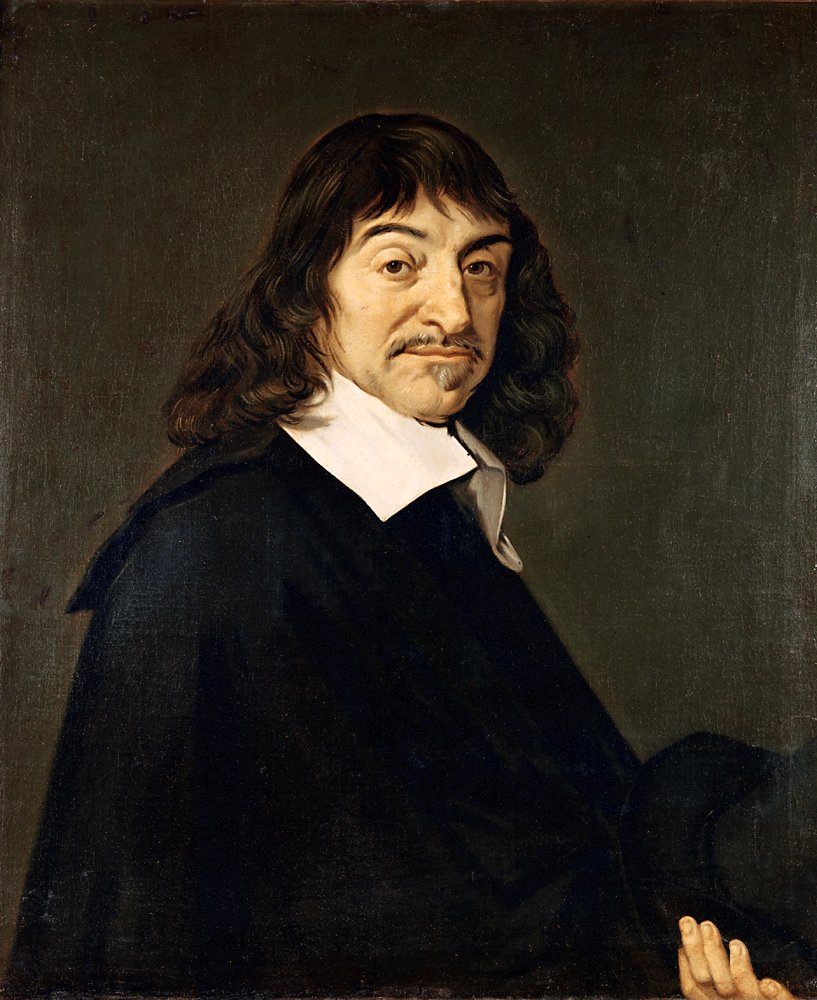
\includegraphics[width=0.9\textwidth]{Cartesian.jpg}
\end{figure}
\end{minipage}
\hfill
\begin{minipage}[b]{0.7\textwidth}
  \hspace{2em}\alertg{Ren\'{e} Descartes} (31 March 1596 -- 11 February 1650) has been dubbed the ``Father of Modern Philosophy''.
  Descartes' influence in mathematics is equally apparent;
  the Cartesian coordinate system was named after him.
  He is credited as the father of analytical geometry,
  the bridge between algebra and geometry, crucial to the discovery of infinitesimal calculus and analysis.
\end{minipage}\pause

\vspace{0.75ex}
He is perhaps best known for the philosophical statement ``\emph{Cogito ergo sum}''
(French: \emph{Je pense, donc je suis}; English: \emph{I think, therefore I am}; or \emph{I am thinking,
therefore I exist} or \emph{I do think, therefore I do exist}; 中文: 我思故我在).
\end{frame}

%==============================================================================%
{\kongbai
\begin{frame}[t]{笛卡儿积}
\pause
\begin{exam}
  设$A=\{0,1\}$,求$A\times P(A)$。
\end{exam}\pause
\vspace{-3ex}
  \[A \times P(A)=\{\langle 0, \emptyset\rangle,\langle 0,\{0\}\rangle,\langle 0,\{ 1\}\rangle,\langle 0,\{ 0,1\}\rangle,\langle 1, \varnothing\rangle,\langle 1,\{ 0\}\rangle,\langle 1,\{ 1\}\rangle,\langle1,\{0,1\}\rangle\}\vspace{-4ex}\]\pause
  \vspace{2ex}
\begin{exam}
  设$A=\{\spadesuit,\cquptred{\varheartsuit},\clubsuit,\cquptred{\vardiamondsuit}\},B=\{{\rm Ace,King,Queen,Jack},10,9,8,7,6,5,4,3,2\}$,则\pause
  \vspace{-1ex}
  \begin{equation*}
    \begin{aligned}
     A\times B=\{
     &\langle \spadesuit,{\rm Ace}\rangle,\langle \spadesuit,{\rm King}\rangle,\langle \spadesuit,{\rm Queen}\rangle,\ldots,\langle \spadesuit,3\rangle,\langle \spadesuit,2\rangle,\\
     & \langle \cquptred{\varheartsuit},{\rm Ace}\rangle,\langle \cquptred{\varheartsuit},{\rm King}\rangle,\langle \cquptred{\varheartsuit},{\rm Queen}\rangle,\ldots,\langle \cquptred{\varheartsuit},3\rangle,\langle \cquptred{\varheartsuit},2\rangle,\\
     &\langle \clubsuit,{\rm Ace}\rangle,\langle \clubsuit,{\rm King}\rangle,\langle \clubsuit,{\rm Queen}\rangle,\ldots,\langle \clubsuit,3\rangle,\langle \clubsuit,2\rangle,\\
     &\langle \cquptred{\vardiamondsuit},{\rm Ace}\rangle,\langle \cquptred{\vardiamondsuit},{\rm King}\rangle,\langle \cquptred{\vardiamondsuit},{\rm Queen}\rangle,\ldots,\langle \cquptred{\vardiamondsuit},3\rangle,\langle \cquptred{\vardiamondsuit},2\rangle\}.
    \end{aligned}
  \end{equation*}
\end{exam}

\end{frame}}

%==============================================================================%
{\kongbai
\begin{frame}{笛卡儿积的性质}
\pause
\begin{block}{}
\begin{itemize}
  \item 当$A\neq\emptyset \land B\neq\emptyset\land A\neq B$时,\alert{$A\times B\neq B\times A$}。
\end{itemize}
\end{block}\pause

因为
\begin{equation*}\begin{array}{l}
A \times B=\{\langle a, b\rangle \mid a \in A \wedge b \in B\}, \\ \pause
B \times A=\{\langle b, a\rangle \mid b \in B \wedge a \in A\}.
\end{array}\end{equation*}\pause
而当$a\neq b$时,序偶$\langle a, b\rangle \neq\langle b, a\rangle$。

\pause
\begin{exam}
  设$A=\{1,2\},B=\{\alpha,\beta\}$,\pause 则
  $$\begin{array}{l}
A \times B=\{\langle 1, \alpha\rangle,\langle 1, \beta\rangle,\langle 2, \alpha\rangle,\langle 2, \beta\rangle\}, \\\pause
B \times A=\{\langle\alpha, 1\rangle,\langle\beta, 1\rangle,\langle\alpha, 2\rangle,\langle\beta, 2\rangle\}
\end{array}.$$\pause
显然$A\times B\neq B\times A$。
\end{exam}
\end{frame}}

%==============================================================================%
\begin{frame}{笛卡儿积的性质}
\pause
\begin{block}{}
\begin{itemize}
  \item 当$A \neq \varnothing \wedge B \neq \varnothing \wedge C \neq \varnothing$时,\alert{$(A \times B) \times C \neq A \times(B \times C)$}。
\end{itemize}
\end{block}\pause

因为
      \begin{equation*}\begin{aligned}
(A \times B) \times C &=\{\langle\langle a, b\rangle, c\rangle \mid \langle a, b\rangle \in A \times B \wedge c \in C\} \\\pause
&=\{\langle a, b, c\rangle \mid a \in A \wedge b \in B \wedge c \in C\}, \\[6pt]\pause
A \times(B \times C) &=\{\langle a,\langle b, c\rangle\rangle \mid a \in A \wedge\langle b, c\rangle \in B \times C\}.
\end{aligned}\end{equation*}\pause

而$\langle a,\langle b, c\rangle\rangle$不是有序三元组,所以$(A \times B) \times C \neq A \times(B \times C)$。

\end{frame}

%==============================================================================%
\begin{frame}{笛卡儿积的性质}
\pause
\begin{defi}
  设$A,B,C$为任意集合,$\ast$表示$\cup$,$\cap$或$-$运算,则下列结论成立:\pause
  \begin{enumerate}
    \item 笛卡尔积对于并、交、差运算可左分配。即 \pause
    $$A \times(B * C)=(A \times B) *(A \times C).\vspace{-4ex}$$ \pause
    \item 笛卡尔积对于并、交、差运算可右分配。即 \pause
    $$(B * C) \times A=(B \times A) *(C \times A).$$
  \end{enumerate}
\end{defi}

\end{frame}
%==============================================================================%

\begin{frame}{笛卡儿积的性质}
\pause
\begin{exam}
  证明$(B \cap C) \times A=(B \times A) \cap(C \times A)$。
\end{exam}\pause
\vspace{1ex}
在集合$(B \cap C) \times A$中任取$\opxy$,\pause 则
\begin{equation*}\begin{array}{ll}
\quad\langle x, y\rangle \in(B \cap C) \times A \\[4pt]\pause
\Leftrightarrow x \in(B \cap C) \wedge y \in A \\[4pt]\pause
\Leftrightarrow(x \in B \wedge x \in C) \wedge y \in A \\[4pt]\pause
\Leftrightarrow x \in B \wedge y \in A \wedge x \in C \wedge y \in A \\[4pt]\pause
\Leftrightarrow(x \in B \wedge y \in A) \wedge(x \in C \wedge y \in A) \\[4pt]\pause
\Leftrightarrow\langle x, y\rangle \in(B \times A) \wedge\langle x, y\rangle \in(C \times A) \\[4pt]\pause
\Leftrightarrow\langle x, y\rangle \in(B \times A) \cap(C \times A).
\end{array}\end{equation*}

\end{frame}

%==============================================================================%

\begin{frame}{笛卡儿积的性质}
\pause
\begin{exam}
证明$(A-B) \times C=(A \times C)-(B \times C)$。
\end{exam}
\pause
\vspace{1ex}
在集合$(A \times C)-(B \times C)$中任取$\opxy$,\pause 则
\begin{equation*}\begin{array}{l}
\quad\langle x, y\rangle \in(A \times C)-(B \times C) \\[2pt]\pause
\Leftrightarrow\langle x, y\rangle \in A \times C \wedge \neg\langle x, y\rangle \in B \times C \\[2pt]\pause
\Leftrightarrow(x \in A \wedge y \in C) \wedge \neg(x \in B \wedge y \in C) \\[2pt]\pause
\Leftrightarrow(x \in A \wedge y \in C) \wedge(\neg x \in B \vee \neg y \in C) \\[2pt]\pause
\Leftrightarrow(x \in A \wedge y \in C \wedge \neg x \in B) \vee(x \in A \wedge y \in C \wedge \neg y \in C) \\[2pt]\pause
\Leftrightarrow(x \in A \wedge y \in C \wedge \neg x \in B) \vee \F \\[2pt]\pause
\Leftrightarrow x \in A \wedge \neg x \in B \wedge y \in C \\[2pt]\pause
\Leftrightarrow x\in(A-B) \wedge y \in C\\[2pt]\pause
\Leftrightarrow \opxy \in (A-B)\times C.
\end{array}\end{equation*}
\end{frame}

%==============================================================================%

\begin{frame}{笛卡儿积的性质}
\pause
\begin{thm}
  若$C\neq \emptyset$,则$A \subseteq B \Leftrightarrow A \times C \subseteq B \times C \Leftrightarrow C \times A \subseteq C \times B$。
\end{thm}
\pause
若$A\subseteq B$,\pause 任取$\opxy \in A\times C$,\pause 有
\begin{equation*}\begin{aligned}
\langle x, y\rangle \in A \times C & \Leftrightarrow x \in A \wedge y \in C \\\pause
& \Rightarrow x \in B \wedge y \in C \pause \Leftrightarrow\langle x, y\rangle \in B \times C.\pause
\end{aligned}\end{equation*}
因此$ A \times C \subseteq B \times C$。

\pause
反之,若$ A \times C \subseteq B \times C$,\pause 任取$x\in A$。 \pause 存在$y\in C$, 使得
\begin{equation*}\begin{aligned}
x \in A & \Leftrightarrow x \in A \wedge y \in C \pause \Leftrightarrow\langle x, y\rangle \in A \times C \pause \Rightarrow\langle x, y\rangle \in B \times C \\ \pause
&\Leftrightarrow x \in B \wedge y \in C\pause
\Leftrightarrow x \in B.
\end{aligned}\end{equation*}\pause
因此$A\subseteq B$。 \pause 类似可以证明$A \subseteq B \Leftrightarrow C \times A \subseteq C \times B$。
\end{frame}

%==============================================================================%

\begin{frame}{笛卡儿积的性质}
\pause
\begin{thm}
  设$A,B,C,D$为四个非空集,则$A \times B \subseteq C \times D \Leftrightarrow A \subseteq C, B \subseteq D$。
\end{thm}\pause
\vspace{1ex}

若$A \times B \subseteq C \times D$,\pause 对任意$x\in A$和$y\in B$,\pause 有
\begin{equation*}
(x \in A) \wedge(y \in B) \pause \Leftrightarrow\langle x, y\rangle \in A \times B \pause
\Rightarrow\langle x, y\rangle \in C \times D \pause
 \Leftrightarrow(x \in C) \wedge(y \in D).
\end{equation*}\pause
因此,$A\subseteq C$且$B\subseteq D$。\pause

反之,若$A\subseteq C$且$B\subseteq D$,\pause 对任意$x\in A$和$y\in B$,\pause 有
\begin{equation*}
\langle x, y\rangle \in A \times B \pause \Leftrightarrow(x \in A) \wedge(y \in B)\pause
 \Rightarrow(x \in C) \wedge(y \in D) \pause
 \Leftrightarrow\langle x, y\rangle \in C \times D.
\end{equation*}\pause
因此,$A \times B \subseteq C \times D$。
\end{frame}

%==============================================================================%
{\kongbai
\begin{frame}{$n$次笛卡尔积}
\pause
  \begin{defi}
    对任意集合$A_1,A_2,\ldots,A_n$,$A_1\times A_2\times \cdots\times A_n$递归地定义为:\pause
    \begin{equation*}
    \begin{aligned}
      A_1\times A_2&=\{\left\langle x_1,x_2\right\rangle\mid x_1\in A_1\wedge x_2\in A_2\},\\ \pause
      A_1\times A_2\times A_3&=\left(A_1\times A_2\right)\times A_3,\\ \pause
      &\cdots\cdots \\
     A_1\times\cdots\times A_{n-1}\times  A_n&=\left(A_1\times\cdots\times A_{n-1}\right)\times A_n,
    \end{aligned}\pause
  \end{equation*}
  即$A_1\times\cdots\times A_{n-1}\times  A_n=\{\left\langle x_1,\ldots ,x_{n-1},x_n\right\rangle\mid x_1\in A_1\land\cdots\land x_{n-1}\in A_{n-1}\land x_n\in A_n\}$。\pause 特别的,$\underbrace{A\times A\times \cdots\times A}_n$简记为$A^n$。
  \end{defi}
\end{frame}
}

%==============================================================================%
\begin{frame}{$n$次笛卡尔积}
\pause
\begin{exam}
  设$A=\{0,1\},B=\{1,2\}$,确定以下集合
  \vspace{-1.5ex}
  \begin{multicols}{4}
  \begin{enumerate}
    \item $A\times \{1\}\times B$;
    \item $A^2\times B$.
  \end{enumerate}
  \end{multicols}
\end{exam}\pause
\vspace{2ex}
\begin{enumerate}
  \item $A \times\{1\} \times B=\{\langle 0,1,1\rangle,\langle 0,1,2\rangle,\langle 1,1,1\rangle,\langle 1,1,2\rangle\}$.\\[6pt] \pause
  \item $A^{2} \times B=\{\langle0,0,1\rangle,\langle 0,1,1\rangle,\langle 0,0,2\rangle,\langle 0,1,2\rangle,\langle 1,0,1\rangle,\langle 1,0,2\rangle,\langle 1,1,1\rangle,\langle 1,1,2\rangle\}$.
\end{enumerate}

\end{frame}

%==============================================================================%
\subsection{二元关系的定义}

\begin{frame}{关系的概念}
\pause
事物之间存在着各式各样的关系. \pause 例如,
\begin{itemize}
  \item 数之间的大小关系($1<2$),整除关系($3|27$); \pause
  \item 人际关系(老乡关系,同学关系 ,亲戚关系)
\end{itemize}
\pause
\begin{exam}
  三名学生$A,B,C$选修$\alpha,\beta,\gamma,\delta$四门课,设$A$选$\alpha$和$\delta$,$B$选$\gamma$,$C$选$\alpha$和$\beta$。\pause
  那么,三名学生选课的对应关系可以概括为:
  \vspace{-1ex}
  $$R=\{\langle A, \alpha\rangle,\langle A, \delta\rangle,\langle B, \gamma\rangle,\langle C, \alpha\rangle,\langle C, \beta\rangle\}.\vspace{-1ex}$$ \pause
  集合$R$反映了学生集合$S=\{A,B,C\}$与课程集合$T=\{\alpha,\beta,\gamma,\delta\}$之间的某种关系。
\end{exam}
\pause
\vspace{1ex}
\finger~集合$R$是笛卡儿积$S\times T$的子集。
\end{frame}

%==============================================================================%

\begin{frame}{二元关系}
\pause
\begin{defi}
  令 $A$和$B$是任意两个集合, 笛卡尔积$A\times B$的子集$R$ 称为$A$到$B$的\alert{二元关系(binary relation)}.\pause
  \begin{enumerate}
    \item $R$中的任一序偶$\opxy$记为$\opxy\in R$,或 \cquptred{$xRy$}。\pause
    \item $(A\times B)-R$中的任一序偶$\opxy$记为$\opxy\notin R$,或 \cquptred{$x\notr y$}。
  \end{enumerate}\pause
  特别的,若$R\subseteq A\times A$,称$R$为\alert{$A$上的二元关系}。
\end{defi}
\end{frame}
%==============================================================================%


\begin{frame}{二元关系}
\pause
\begin{exam}
  设$A=\{a,b\}$,$B=\{2,5,8\}$,则 \pause
  $$A \times B=\{\langle a, 2\rangle,\langle a, 5\rangle,\langle a, 8\rangle,\langle b, 2\rangle,\langle b, 5\rangle,\langle b, 8\rangle\}.$$ \pause
  令
  $$R_{1}=\{\langle a, 2\rangle,\langle a, 8\rangle,\langle b, 2\rangle\}, \pause
  R_{2}=\{\langle a, 5\rangle,\langle b, 2\rangle,\langle b, 5\rangle\}, \pause
  R_{3}=\{\langle a, 2\rangle\}.$$\pause
  因为$R_1\in A\times B,R_2\in A\times B,R_3\in A\times B$,\pause
  所以$R_1,R_2,R_3$均是$A$到$B$的关系。
\end{exam}

\end{frame}

%==============================================================================%

\begin{frame}{二元关系}
\pause
\begin{exam}
设$A=\{1,2,3,4\}$,确定$A$上的“小于等于”关系$L_A$及“整除关系”$D_A$。
\end{exam}
\pause
\begin{equation*}\begin{aligned}
L_{A} &=\{\langle x, y\rangle \mid \langle x, y\rangle\in A\times A \wedge x \leqslant y\} \\ \pause
&=\{\langle 1,1\rangle,\langle 1,2\rangle,\langle 1,3\rangle,\langle 1,4\rangle,\langle 2,2\rangle,\langle 2,3\rangle,\langle 2,4\rangle,\langle 3,3\rangle,\langle 3,4\rangle,\langle 4,4\rangle\}.\\[10pt]\pause
D_{A} &=\{\langle x, y\rangle \mid \langle x, y\rangle\in A\times A\wedge y/x\in\mathbf{Z}\} \\ \pause
&=\{\langle 1,1\rangle,\langle 1,2\rangle,\langle 1,3\rangle,\langle 1,4\rangle,\langle 2,2\rangle,\langle 2,4\rangle,\langle 3,3\rangle,\langle 4,4\rangle\}.
\end{aligned}\end{equation*}

\end{frame}
%==============================================================================%

\begin{frame}{特殊的二元关系}
\pause
\begin{rem}
\begin{itemize}
  \item 因为$\emptyset\subseteq A\times B$,$\emptyset\subseteq A\times A$,所以$\emptyset$是$A$到$B$的关系,也是$A$上的关系,称为\alert{空关系(empty relation)}。\\[8pt]\pause

  \item 因为$A\times B\subseteq A\times B$,$A\times A\subseteq A\times A$,所以$A\times B$是一个$A$到$B$的关系,称为\alert{全域关系(universal relation)}。$A\times A$是$A$上的全域关系,记为$E_A$。\\[8pt]\pause

  \item $I_A=\{\langle a,a\rangle\mid a\in A\}$为$A$上的\alert{恒等关系(identity relation)}。
\end{itemize}
\end{rem}

\end{frame}

%==============================================================================%
\subsection{二元关系的表示}
\begin{frame}{集合表示}
\pause
\begin{itemize}
  \item 由于关系也是一种特殊的集合,所以集合的两种基本的表示法也可以用到关系的表示中。即可用列举法和描述法来表示关系 。
\end{itemize}\pause
\vspace{2ex}
\begin{description}
  \item[列举法:] $L_{A} =\{\langle 1,1\rangle,\langle 1,2\rangle,\langle 1,3\rangle,\langle 1,4\rangle,\langle 2,2\rangle,\langle 2,3\rangle,\langle 2,4\rangle,\langle 3,3\rangle,\langle 3,4\rangle,\langle 4,4\rangle\}.$ \\[6pt]\pause
  \item[描述法:] $D_A=\{\opxy\mid \opxy\in A\times A\land y/x\in\mathbf{Z}\}$.
\end{description}

\end{frame}

%==============================================================================%

\begin{frame}{矩阵表示}
\pause
\begin{defi}
  给定两个有限集合$A=\{a_1,a_2,\ldots,a_n\}$, $B=\{b_1,b_2,\ldots,b_m\}$。 设$R$为从$A$到$B$的一个二元关系。则对应于关系$R$的\alert{关系矩阵(relation matrix)}为矩阵$M_R=(r_{ij})_{n\times m}$,\pause  其中
  $$r_{i j}=\left\{\begin{array}{ll}
1, & \left\langle a_{i}, b_{j}\right\rangle \in R, \\[3pt]
0, & \left\langle a_{i}, b_{j}\right\rangle \notin R.
\end{array}\right.$$\pause
特别地,当$R$为集合$A$上的关系时,$M_R$为方阵。
\end{defi}
\end{frame}

%==============================================================================%

\begin{frame}{矩阵表示}

\pause
\begin{exam}
  设集合$A=\{1,2,3,4,5\}$,$B=\{a,b,c\}$,则关系$R=\{\langle1,a\rangle,\langle 2,b\rangle,\langle 3,a\rangle\}$对应的关系矩阵为:\pause

\renewcommand{\kbldelim}{(}
\renewcommand{\kbrdelim}{)}
$$
\only<3>{
M_R=\kbordermatrix{&a&b&c\\
1&1&0&0\\
2&0&1&0\\
3&1&0&0\\
4&0&0&0\\
5&0&0&0
}}
\only<4->{
M_R=\left(
  \begin{array}{ccc}
    1 & 0 & 0 \\
    0 & 1 & 0 \\
    1 & 0 & 0 \\
    0 & 0 & 0 \\
    0 & 0 & 0 \\
  \end{array}
\right).}$$
\end{exam}
\end{frame}
%==============================================================================%

\begin{frame}[t]{矩阵表示}
\pause
\begin{exam}
  设$P=\{0,1,2,3,4,5,6\}$上的二元关系为$R=\{\opxy\mid x<y\lor x是素数\}$,写出关系矩阵。
\end{exam}
\pause
因为$P$中的素数元素有$ 2, 3, 5$; 又注意到命题联接词$\lor$, \pause
得关系矩阵为:
$$M_{R}=\left(\begin{array}{ccccccc}
0 & 1 & 1 & 1 & 1 & 1 & 1 \\
0 & 0 & 1 & 1 & 1 & 1 & 1 \\
1 & 1 & 1 & 1 & 1 & 1 & 1 \\
1 & 1 & 1 & 1 & 1 & 1 & 1 \\
0 & 0 & 0 & 0 & 0 & 1 & 1 \\
1 & 1 & 1 & 1 & 1 & 1 & 1 \\
0 & 0 & 0 & 0 & 0 & 0 & 0
\end{array}\right)$$
\end{frame}

%==============================================================================%
{\kongbai
\begin{frame}[t]{矩阵表示}
\addtocounter{exam}{-1}
\begin{exam}
  设$P=\{0,1,2,3,4,5,6\}$上的二元关系为$R=\{\opxy\mid x<y\lor x是素数\}$,写出关系矩阵。
\end{exam}
\pause
若设$R_1=\{\opxy\mid x<y\},R_2=\{\opxy\mid  x是素数\}$。\pause 则对应的关系矩阵分别为:
{\small
$$M_{R_{1}}=\left(\begin{array}{ccccccc}
0 & 1 & 1 & 1 & 1 & 1 & 1 \\
0 & 0 & 1 & 1 & 1 & 1 & 1 \\
0 & 0 & 0 & 1 & 1 & 1 & 1 \\
0 & 0 & 0 & 0 & 1 & 1 & 1 \\
0 & 0 & 0 & 0 & 0 & 1 & 1 \\
0 & 0 & 0 & 0 & 0 & 0 & 1 \\
0 & 0 & 0 & 0 & 0 & 0 & 0
\end{array}\right), \quad \pause M_{R_{2}}=\left(\begin{array}{ccccccc}
0 & 0 & 0 & 0 & 0 & 0 & 0 \\
0 & 0 & 0 & 0 & 0 & 0 & 0 \\
1 & 1 & 1 & 1 & 1 & 1 & 1 \\
1 & 1 & 1 & 1 & 1 & 1 & 1 \\
0 & 0 & 0 & 0 & 0 & 0 & 0 \\
1 & 1 & 1 & 1 & 1 & 1 & 1 \\
0 & 0 & 0 & 0 & 0 & 0 & 0
\end{array}\right).$$}\pause
若规定$M_{R_1}\lor M_{R_2}$为对应元素作$\lor$运算,\pause
则$M_{R_1}\lor M_{R_2}=M_R$。
\end{frame}}
%==============================================================================%

\begin{frame}{关系图表示}
\pause
\begin{defi}
  给定两个有限集合$A=\{a_1,a_2,\ldots,a_n\}$, $B=\{b_1,b_2,\ldots,b_m\}$。 设$R$为从$A$到$B$的一个二元关系。$R$的\alert{关系图(relation digraph)}~$G_R$由如下方法定义:\pause
  \begin{enumerate}
    \item 在平面上作出$n$个\alert{结点(node)}代表$A$,分别记作$a_1,a_2,\ldots,a_n$;\pause
    \item 再在平面上作出$m$个\alert{结点(node)}代表$B$,分别记作$b_1,b_2,\ldots,b_m$;\pause
    \item 如果$\langle a_i,b_j \rangle\in R$,则自结点$a_i$到结点$b_j$作出一条\alert{有向边(direct edge)},其箭头指向$b_j$。\pause
        如果$\langle a_i,b_j \rangle\notin R$,则结点$a_i$和结点$b_j$之间没有线段联结。
  \end{enumerate}
\end{defi}
\end{frame}

%==============================================================================%
\begin{frame}[t]{关系图表示}
\pause
\begin{exam}
  设集合$A=\{1,2,3,4,5\}$,$B=\{a,b,c\}$,则关系$R=\{\langle1,a\rangle,\langle 2,b\rangle,\langle 3,a\rangle\}$对应的关系图为:
  \pause
\begin{figure}
  \centering
  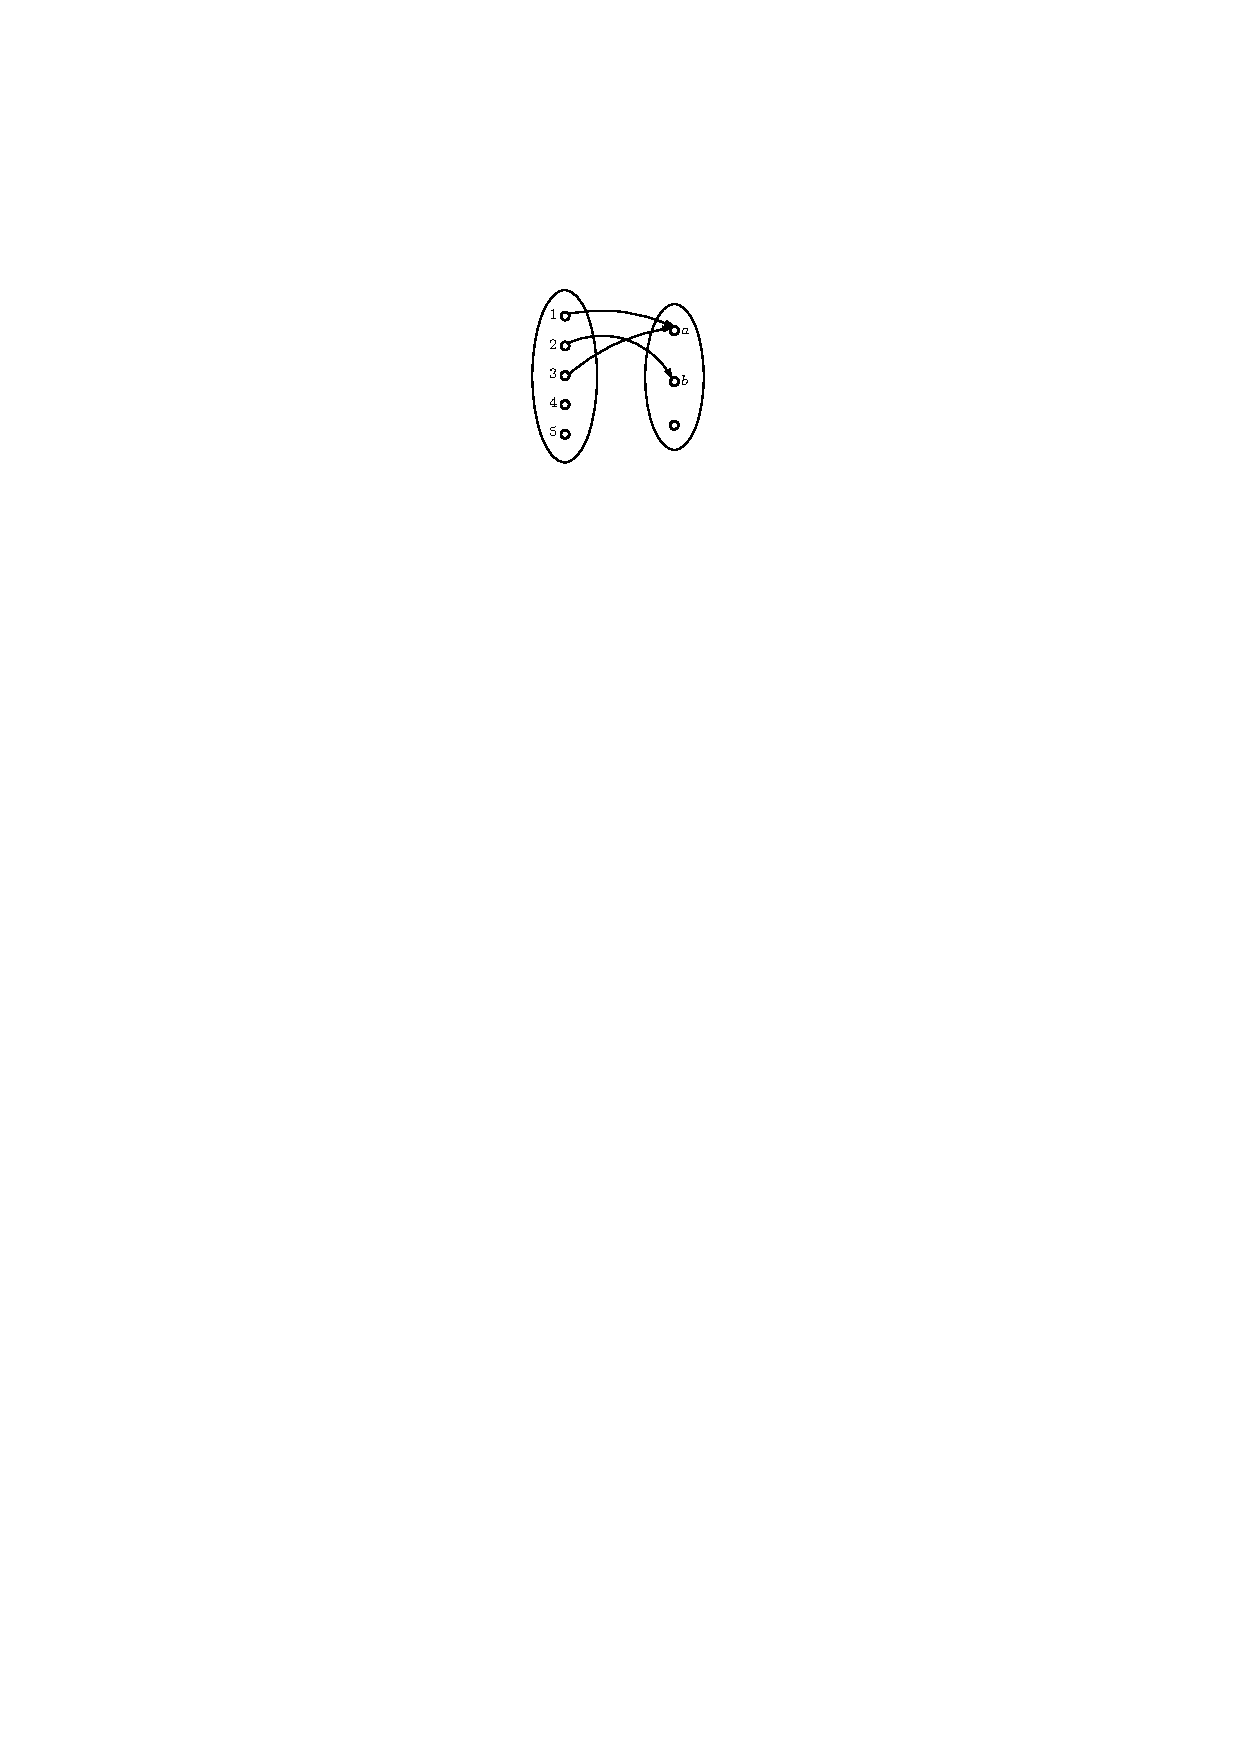
\includegraphics[width=0.24\textwidth]{gr.pdf}
\end{figure}
\end{exam}
\end{frame}

%==============================================================================%
\begin{frame}{关系图表示}
\pause
\begin{exam}
  设$A=\{a,b,c,d\}$上的关系$R=\{\langle a,a\rangle,\langle a,b\rangle,\langle a,c\rangle,\langle b,c\rangle,\langle d,c\rangle,\langle d,d\rangle\}$,画出关系图。
\end{exam}
\pause
\vspace{1ex}
\begin{itemize}
  \item 对于集合$A$上的关系$R$,$G_R$可以仅以$A$的元素为顶点作出。 \pause
\end{itemize}

\begin{figure}
  \centering
  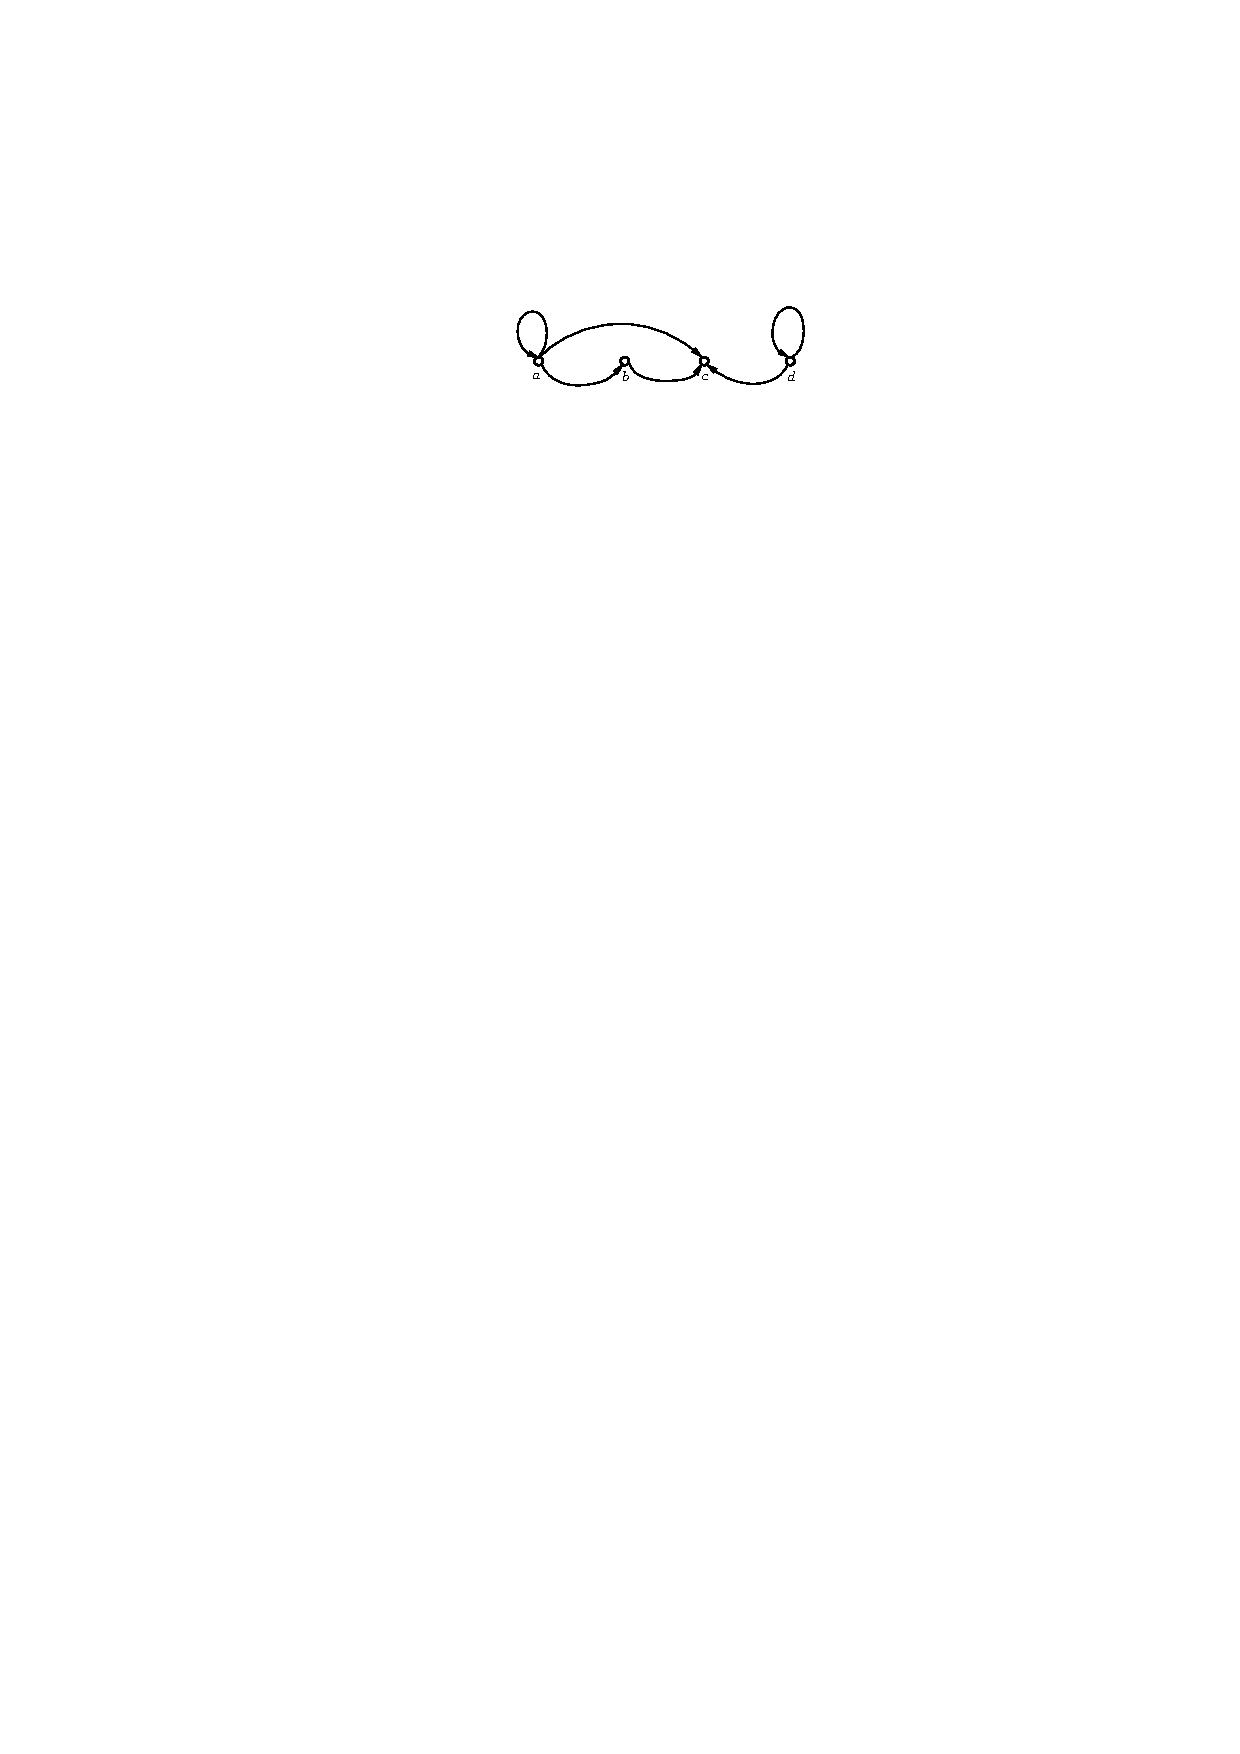
\includegraphics[width=0.47\textwidth]{gr2.pdf}
\end{figure}
\pause
\finger 起点和终点重合的有向边,称为\alert{环(loop)}。

\end{frame} 